%\begin{center}
%	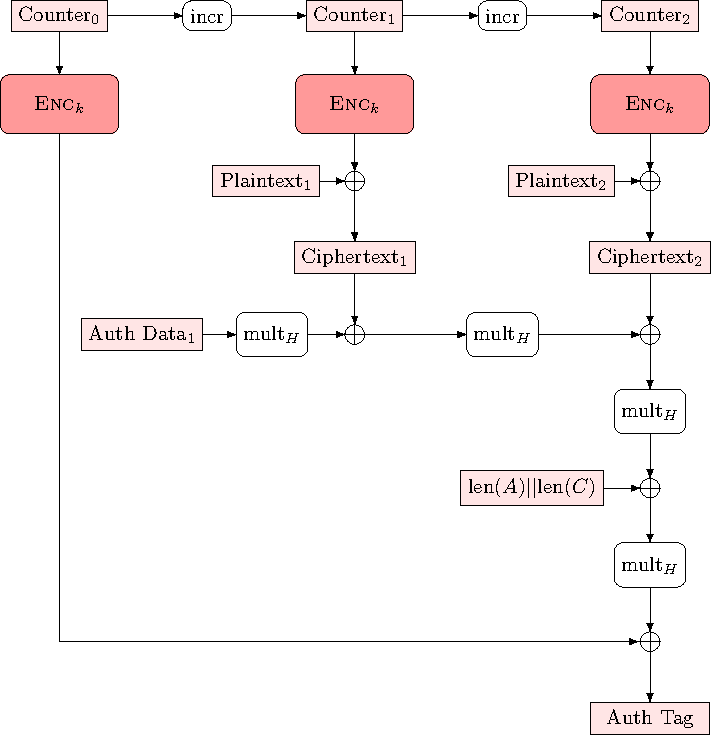
\includegraphics[scale=1]{tikz/GCM_encryption}
%\end{center}

\begin{figure}[h!]\centering
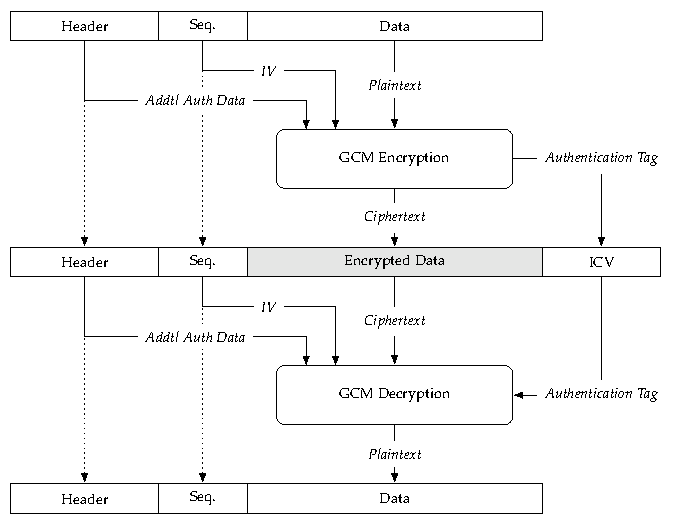
\includegraphics[scale=1.25]{tikz/gcm_mode}
\end{figure}

\subsection{Multiplication in $\GF(2^{128})$}
\begin{definition}
	Let \(\mathbb F_2 = \{0,1\}\) be the field with two elements.  Fix an irreducible polynomial
	\[
	f(x) \;=\; x^{128} + x^7 + x^2 + x + 1 
	\quad\in\; \mathbb F_2[x].
	\]
	Then
	\[
	\mathrm{GF}(2^{128}) \;=\; \mathbb F_2[x] \,\big/\,\bigl(f(x)\bigr)
	\]
	is the degree-\(128\) extension field.
\end{definition}
\begin{remark}
Every element \(\alpha\in\mathrm{GF}(2^{128})\) can be written uniquely as \[
\alpha \;=\; a_{127}x^{127} + a_{126}x^{126} + \cdots + a_1 x + a_0
\quad(a_i\in\{0,1\}).
\] We identify \(\alpha\) with the \(128\)-bit vector \((a_{0},\dots,a_{127})\in\F_2\).
\end{remark}

\paragraph{Polynomial Representation and Reduction}
Multiplication in \(\mathbb F_2[x]\) is carry-less:
\[
\left(\sum_i a_i x^i\right)\cdot\left(\sum_j b_j x^j\right)
=\sum_{i,j}\left(a_i b_j\right)\,x^{i+j}\,,
\]
with all additions mod 2.  To get the product in \(\mathrm{GF}(2^{128})\), we then reduce
the degree-\(\le 254\) result modulo \(f(x)\).

\paragraph{Bit-Level Algorithm}
We implement multiplication by a simple “shift-and-add” method with reduction on each
shift, often called \(\mathtt{xtime}\).

\begin{definition}[\,\(\mathtt{xtime}\) map\,]
	For \(v\in\mathrm{GF}(2^{128})\) represented as a 128-bit word, define
	\[
	\mathtt{xtime}(v) = 
	\begin{cases}
		v \ll 1, &\text{if the MSB of }v\text{ is }0,\\[6pt]
		(v \ll 1)\oplus R, &\text{if the MSB of }v\text{ is }1,
	\end{cases}
	\]
	where \(R\) is the bit-vector corresponding to the reduction polynomial
	\(x^7+x^2+x+1\).
\end{definition}

\paragraph{Pseudocode}
\ \\ \begin{algorithm}[H]
	\caption{Multiply two field elements \(a,b\in\mathrm{GF}(2^{128})\)}
	\label{alg:mul2}
	\begin{algorithmic}[1]
		\REQUIRE \(a,b\in\{0,1\}^{128}\) as 128-bit words  
		\ENSURE \(c = a\cdot b \bmod f(x)\)
		\STATE \(c \leftarrow 0\)  
		\STATE \(v \leftarrow a\)  
		\FOR{\(i=0\) to \(127\)}  
		\IF{bit \(i\) of \(b\) is 1}  
		\STATE \(c \leftarrow c \oplus v\)  
		\ENDIF  
		\STATE \(v \leftarrow \mathtt{xtime}(v)\)  
		\ENDFOR  
		\RETURN \(c\)
	\end{algorithmic}
\end{algorithm}



\paragraph{References:} 
\cite{NIST80038d},\;
\cite{McGrewViega2004gcm}